\documentclass[a4paper,12pt]{article}
\usepackage[top = 3cm, bottom = 2cm, left = 3cm, right=2cm]{geometry}
\usepackage[utf8]{inputenc}
\usepackage{amsmath,amsfonts,amssymb}
\usepackage{float}
\usepackage{graphicx}
\usepackage[brazilian]{babel}
\usepackage{indentfirst}
\usepackage{float}
\usepackage{textcomp}
\usepackage{gensymb}

\title{Documentação MCD - ARAM}

\begin{document}
	\maketitle
	\section{Desenvolvimento da MCD}
	Considerando o diâmetro solar aparente na abóboda celeste como sendo de $2^{\circ}$ (FOV), o diâmetro de um LDR de 4mm (R) e tomando como desenho base a figura 1, os seguintes cálculos foram desenvolvidos: 

\begin{figure}[htb] 
	\centering
	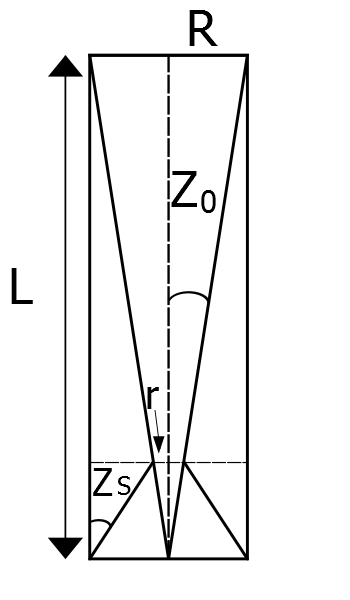
\includegraphics[scale=0.5]{MCD_1.jpg}
	\caption{Primeira versão de um tubo da matriz de sensores.}
\end{figure}

$$\frac{R}{L} = tan(Z_{0}) ; \,\,   R = \frac{D_{LDR}}{2}, Z_{0} = \frac{FOV}{2}$$
$$L = \frac{R}{tan(Z_{0})} \longrightarrow L = \frac{2}{tan(1^{o})}  \longrightarrow L \cong 115 mm$$ 


Notou-se que o comprimento deste tubo foi muito desproporcional, portanto foi necessário adicionar o parâmetro $Z_{s}$ ao tubo, permitindo a conservação do FOV tubo e a redução de seu comprimento em quase 50\%, características que facilitariam na prototipagem rápida em plástico resistente e na proporcionalidade do modelo. Os cálculos dessa etapa seguem abaixo.

\newpage
$$Tan(Z_{s}) = \frac{(R-r)}{L_{novo}}  \, ; \,  onde: \, r= \,1mm \,e \, L_{novo}= \, 60mm $$
$$Tan(Z_{s}) = \frac{(2-1)}{60}  \longrightarrow   Z_{s} = Tan^{-1}(0,0167) \therefore Z_{s} \cong 1^{\circ} $$

Uma vez tendo dimensionado cada tubo de forma individual, outro problema encontrado foi o de ter mais de um sensor localizando o sol ao mesmo tempo, algo que dificultaria a implementação do algoritmo de apontamento fino. A fim de sanar esta problemática desenvolveu-se a MCD(Matriz Circular Detectora), composta pelos mesmos 25 tubos, agora dispostos na superfície de uma calota esférica. Os parâmetros calculados abaixo dizem respeito ao raio da seção transversal(X), Distância do centro da esfera até o início da MCD (d), o tamanho de flecha (F) e o FOV sólido da matriz.
\begin{figure}[htb] 
	\centering
	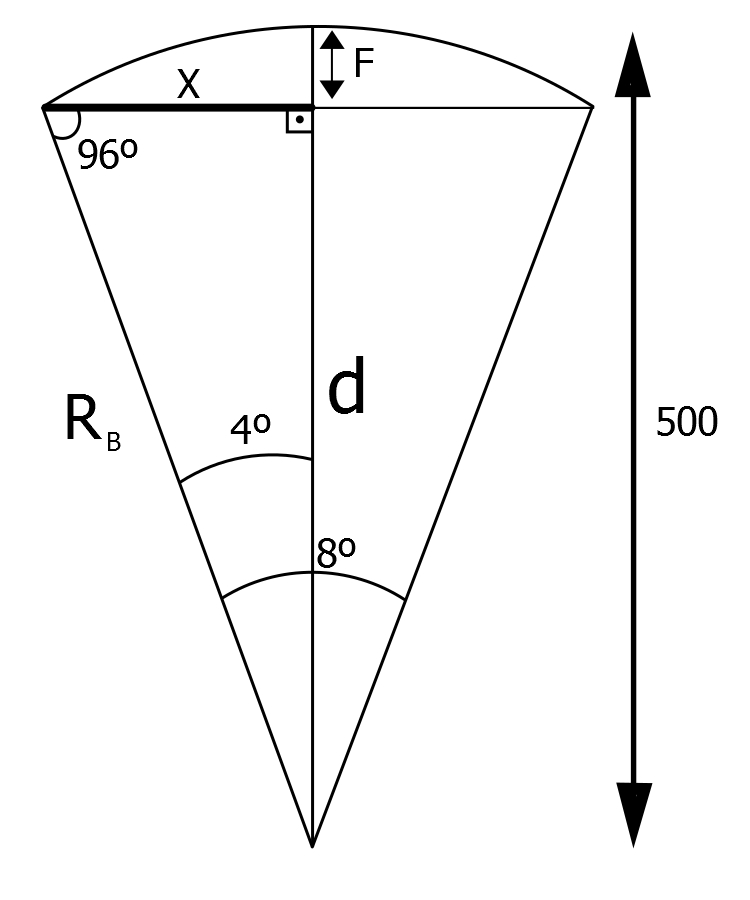
\includegraphics[scale=0.3]{MCD_2.jpg}
	\caption{MCD.}
\end{figure}
$$ \frac{X}{sin(4^{\circ})} = \frac{R_{B}}{sin(90^{\circ})}\longrightarrow X= \frac{R_{B}\times sin(4^{\circ})}{sin(90^{\circ})} \longrightarrow X=\frac{500\times 0,06975}{1} \therefore X=34,87mm $$
$$d = \sqrt{500^{2} - 34,87^{2}} \therefore d=498,78mm \, ;\, F=500-498,78 \therefore F=1,22mm $$

A

\end{document}